\begin{figure}[htbp]
    \centering
    \begin{subfigure}[t]{\textwidth}
        \centering
        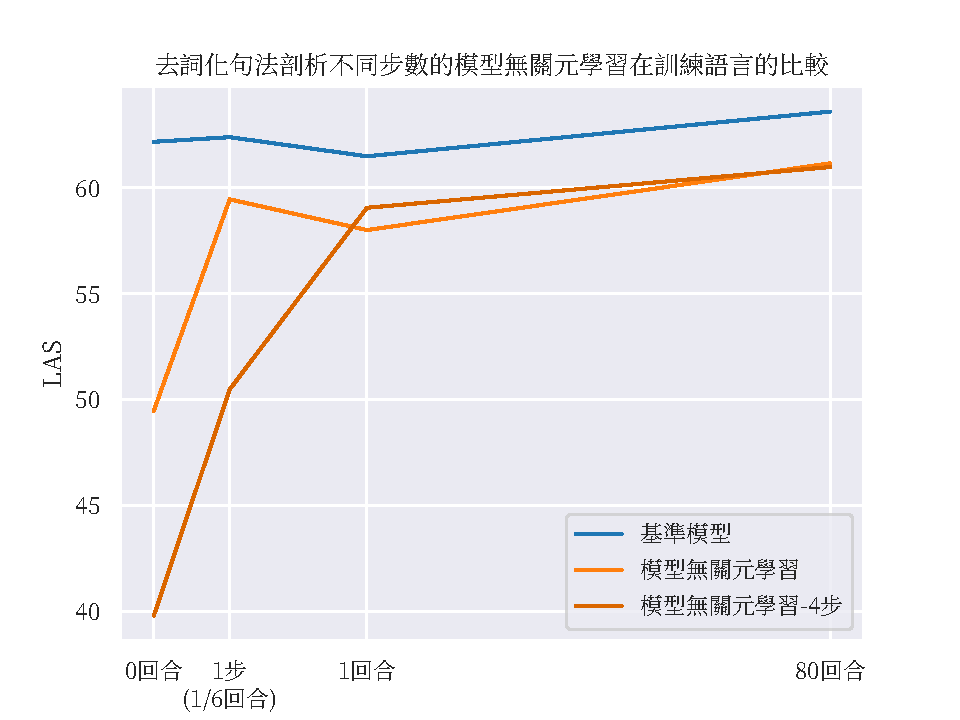
\includegraphics[width=\textwidth]{figs/delex_parsing/linecharts/delex_maml_train_langs.pdf}
    \end{subfigure}
    \vspace{-12pt}
    \begin{subfigure}[t]{\textwidth}
        \centering
        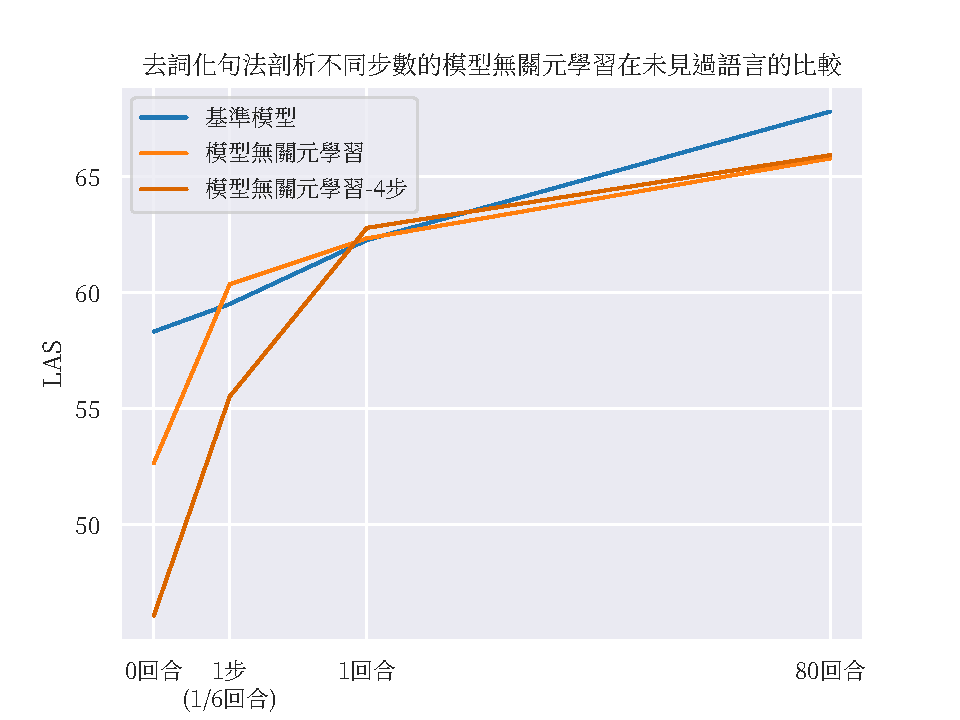
\includegraphics[width=\textwidth]{figs/delex_parsing/linecharts/delex_maml_test_langs.pdf}
    \end{subfigure}
    \caption{去詞化依存句法剖析不同步數的模型無關元學習精細校正後的平均LAS折線圖。}
    \label{fig:delex_avg_maml}
\end{figure}
\begin{figure}[htbp]
    \centering
    \begin{subfigure}[t]{\textwidth}
        \centering
        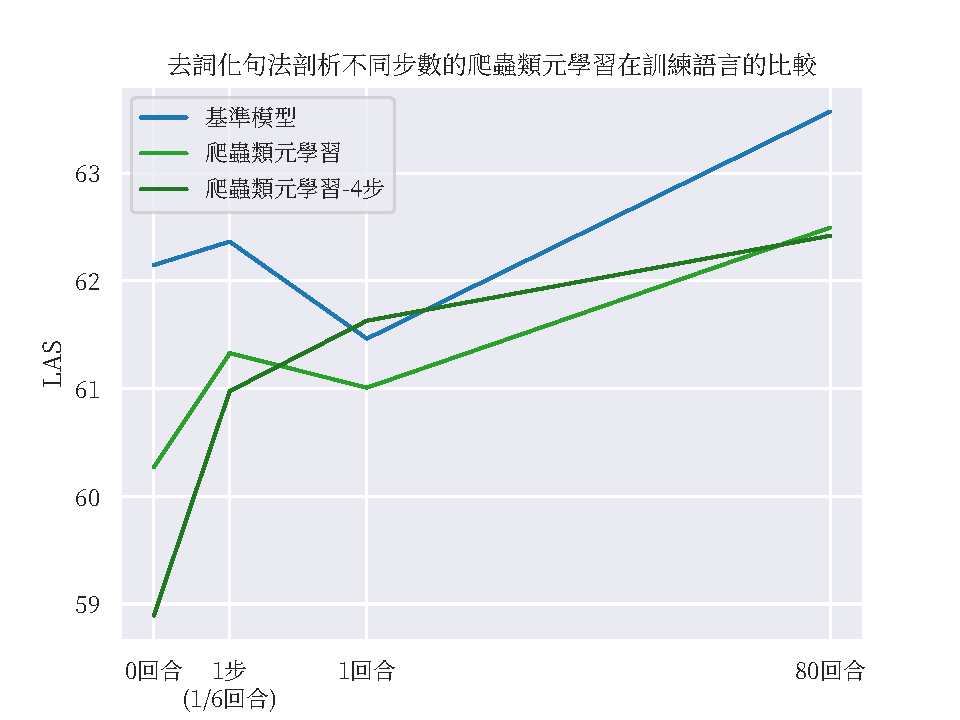
\includegraphics[width=\textwidth]{figs/delex_parsing/linecharts/delex_reptile_train_langs.pdf}
    \end{subfigure}
    \vspace{-12pt}
    \begin{subfigure}[t]{\textwidth}
        \centering
        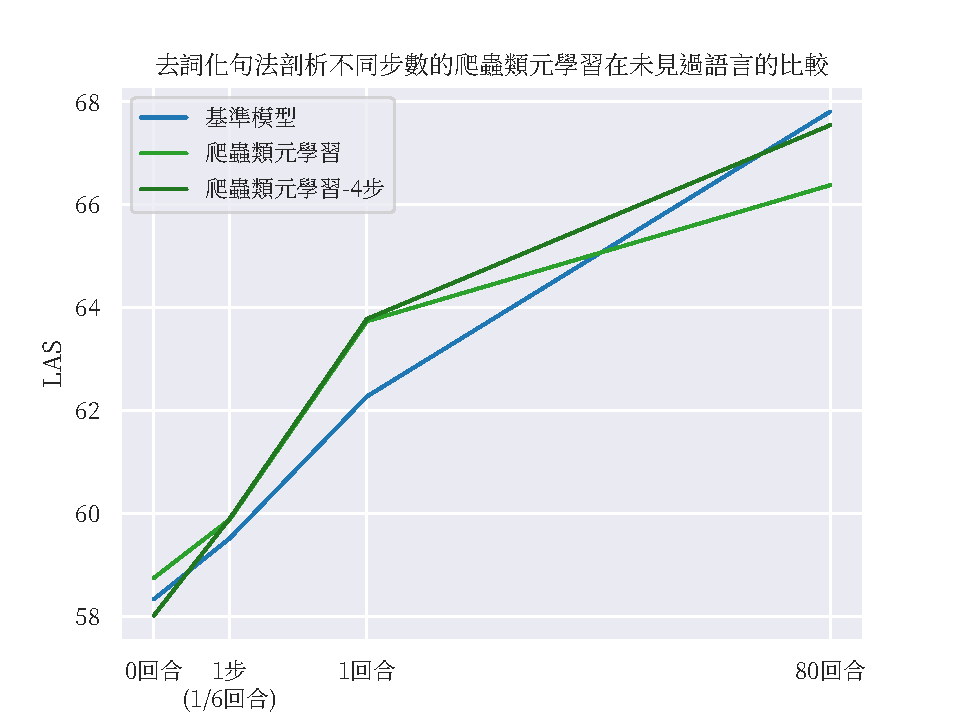
\includegraphics[width=\textwidth]{figs/delex_parsing/linecharts/delex_reptile_test_langs.pdf}
    \end{subfigure}
    \caption{去詞化依存句法剖析不同步數的爬蟲類元學習精細校正後的平均LAS折線圖。}
    \label{fig:delex_avg_reptile}
\end{figure}
\begin{figure}[htbp]
    \centering
    \begin{subfigure}[t]{\textwidth}
        \centering
        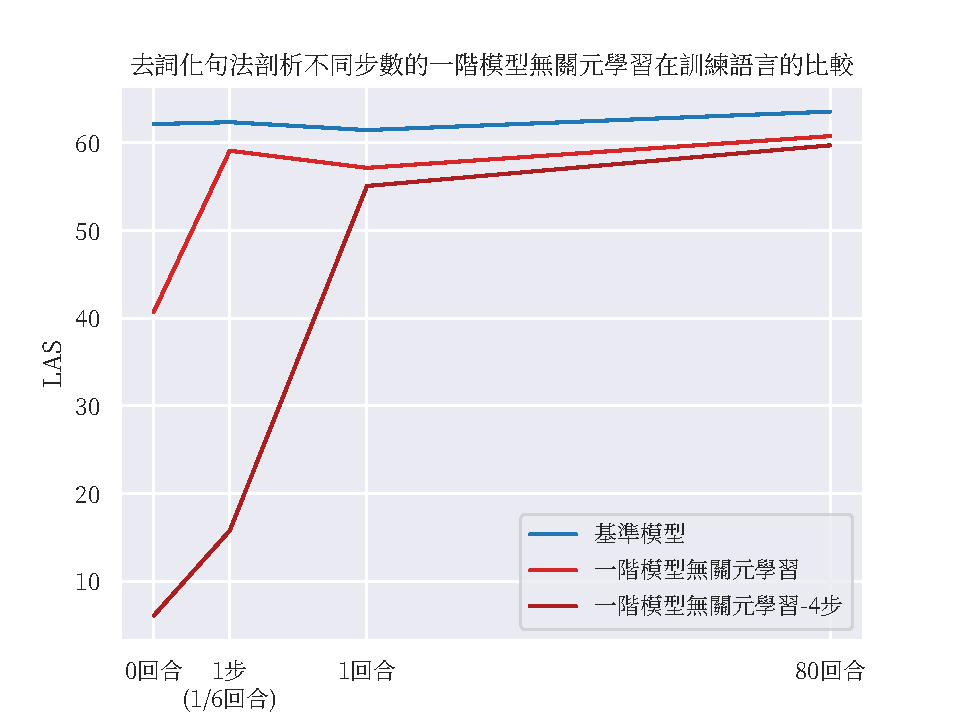
\includegraphics[width=\textwidth]{figs/delex_parsing/linecharts/delex_fomaml_train_langs.pdf}
    \end{subfigure}
    \vspace{-12pt}
    \begin{subfigure}[t]{\textwidth}
        \centering
        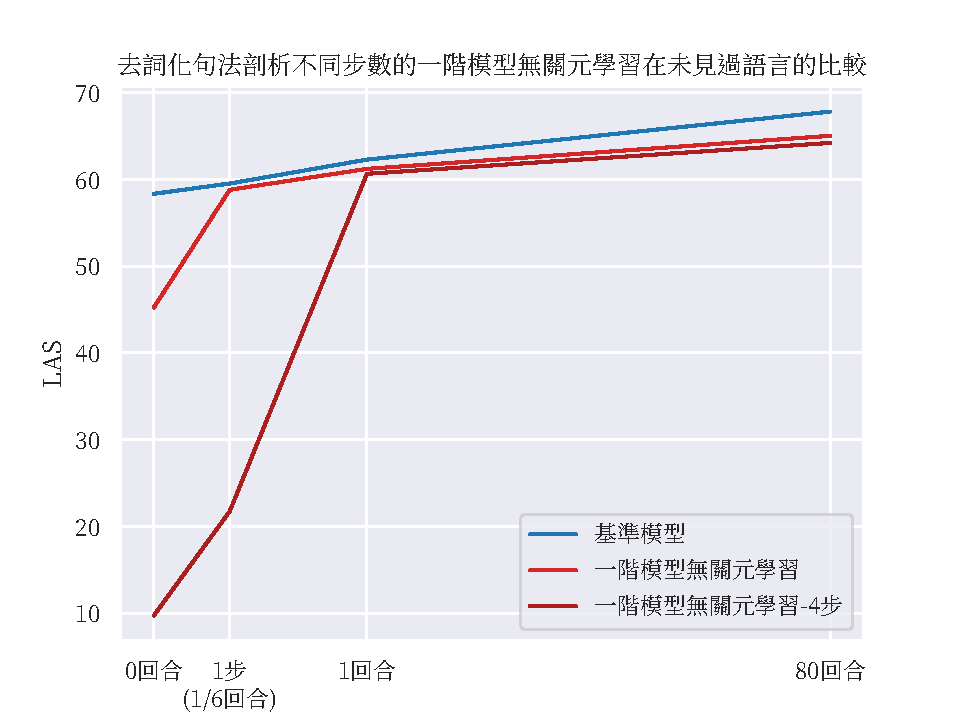
\includegraphics[width=\textwidth]{figs/delex_parsing/linecharts/delex_fomaml_test_langs.pdf}
    \end{subfigure}
    \caption{去詞化依存句法剖析不同步數的一階模型無關元學習精細校正後的平均LAS折線圖。}
    \label{fig:delex_avg_fomaml}
\end{figure}
